% Feature coverage for faster-beamer:
% - explicit table of contents frame (useful to compare preview mode against --unite)
% - \AtBeginSection roadmap frames generated from section hooks
% - nested \input and \include dependencies
% - \graphicspath + \includegraphics on a checked-in EPS asset
% - fragile frame content, cross references, BibTeX, and TikZ
%
% Suggested runs:
%   cargo run -- test/feature-tour.tex --unite --multi-pass=2 --bibliography bibtex --tree-sitter
%   cargo run -- test/feature-tour.tex --watch --unite --multi-pass=2 --bibliography bibtex
%   cargo run -- test/feature-tour.tex --output test/feature-tour-preview.pdf
%
% This commented line is intentional: the dependency scanner should ignore it.
% \input{ignored-by-comment-stripper}

\documentclass[aspectratio=169]{beamer}
\usetheme{Madrid}
\usecolortheme{seagull}

\usepackage[T1]{fontenc}
\usepackage{graphicx}
\usepackage{booktabs}
\usepackage{tikz}
\usepackage{epstopdf}
\usetikzlibrary{arrows.meta,calc,positioning}

\graphicspath{{figures/}}

\title{faster-beamer Feature Tour}
\subtitle{Regression deck for preview, caching, and unite mode}
\author{Repository fixture}
\date{\today}

\AtBeginSection[]
{
  \begin{frame}{Section Roadmap}
    The section hook should create a roadmap slide whenever a new section starts.

    \tableofcontents[currentsection]
  \end{frame}
}

\begin{document}

\begin{frame}
  \titlepage
\end{frame}

\begin{frame}{Agenda}
  This slide checks how explicit TOC content behaves in preview mode versus \texttt{--unite}.

  \tableofcontents
\end{frame}

\section{Caching and Inputs}

\begin{frame}{Input files and overlays}
  \label{frm:nested-input}

  This frame pulls content from multiple external input files.

\begin{itemize}
  \item The first-level content lives in \texttt{sections/intro-body.tex}.
  \item Another root-relative \texttt{\string\input} follows right after this block.
\end{itemize}

\pause

\begin{block}{Why this matters}
Editing either input file should invalidate this frame and refresh the cached PDF.
\end{block}
  \begin{alertblock}{Nested detail}
The dependency scanner should resolve nested \texttt{\string\input} paths relative to the parent file.
\end{alertblock}
\end{frame}

\begin{frame}{Graphics, tables, and counters}
  \label{frm:graphic}

  \begin{columns}[T,onlytextwidth]
    \begin{column}{0.58\textwidth}
      \begin{itemize}
        \item External graphic loaded through \texttt{\string\graphicspath}.
        \item Table content that is easy to diff visually.
        \item Label target for later cross references.
      \end{itemize}

      \begin{tabular}{@{}llr@{}}
        \toprule
        Feature & Mode & Status \\
        \midrule
        Cache & preview & fast \\
        Unite & final & accurate \\
        TOC & frame-only & inspect \\
        \bottomrule
      \end{tabular}
    \end{column}
    \begin{column}{0.38\textwidth}
      \centering
      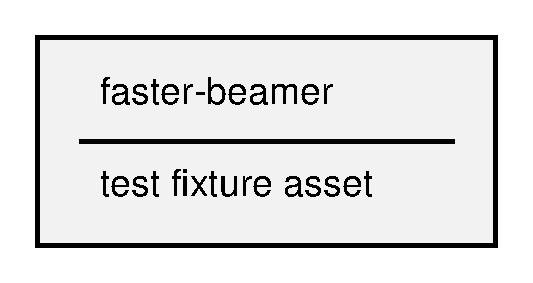
\includegraphics[width=\linewidth]{faster-box}
    \end{column}
  \end{columns}
\end{frame}

\begin{frame}[fragile]{Fragile content}
This frame checks extraction of verbatim-heavy content.

\begin{verbatim}
cargo run -- test/feature-tour.tex --watch --unite --multi-pass=2
cargo run -- test/feature-tour.tex --frame-numbers --parallel --jobs 2
\end{verbatim}
\end{frame}

\section{Cross References and TikZ}

\begin{frame}{Cross references}
The graphic slide is frame~\ref{frm:graphic}.
The nested input slide is frame~\ref{frm:nested-input}.
We also cite \cite{knuth1984texbook} here to exercise BibTeX.
\end{frame}

\begin{frame}{TikZ overview}
  \centering
  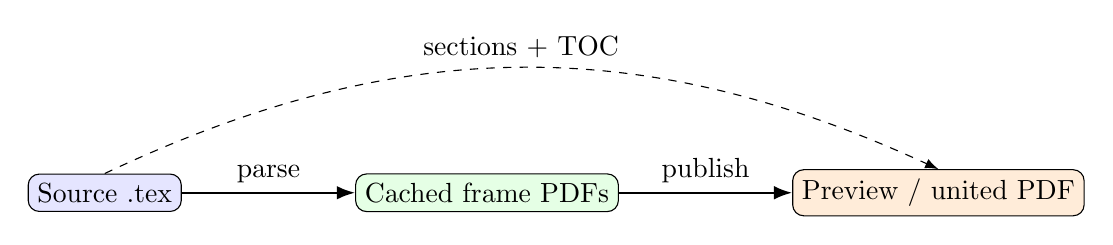
\begin{tikzpicture}[>=Latex, node distance=22mm]
    \node[draw, rounded corners, fill=blue!10] (source) {Source .tex};
    \node[draw, rounded corners, right=of source, fill=green!10] (cache) {Cached frame PDFs};
    \node[draw, rounded corners, right=of cache, fill=orange!15] (output) {Preview / united PDF};

    \draw[->, thick] (source) -- node[above] {parse} (cache);
    \draw[->, thick] (cache) -- node[above] {publish} (output);
    \draw[->, dashed, bend left=25] (source.north) to node[above] {sections + TOC} (output.north);
  \end{tikzpicture}

  \vspace{1em}
  Cross references and some TikZ setups are a good reason to run with \texttt{--multi-pass=2}.
\end{frame}

\section{Included File}

\begin{frame}{Included file}
  This frame comes from \texttt{\string\include\{include-demo\}}.

  \begin{enumerate}
    \item It exercises dependency tracking for a separate source file.
    \item It is useful for cache invalidation checks during \texttt{--watch}.
    \item It gives \texttt{--unite} another nontrivial frame to stitch back together.
  \end{enumerate}
\end{frame}

\appendix
\section{Appendix}

\begin{frame}{Appendix note}
  The appendix adds another section boundary for TOC and frame-number checks.
\end{frame}

\begin{frame}[allowframebreaks]{References}
  This frame stays non-empty even when BibTeX is disabled, which keeps united-mode PDF inclusion valid.

  \bibliographystyle{plain}
  \bibliography{refs}
\end{frame}

\end{document}